%section 1
%%%%%%%%%%%%%%%%%%%%%%%%%%%%%%%%%%%%%%%%%%%%%%%%%%%%%%%%%%%%%%%%%%%%%%%%%%%%%%%%
%%%%%%%%%%%%%%%%%%%%%%%%%%%%%%%%%%%%%%%%%%%%%%%%%%%%%%%%%%%%%%%%%%%%%%%%%%%%%%%%

\section{まず使ってみましょう}\label{sec:triaez}
細かいことは抜きにして、まずは「とりあえず使えるようになる」ことを目指し
ます。
\subsection{\textbf{Overleaf}の準備}\label{sec:overleaf}
今年の演習では\textbf{Overleaf}というオンライン{\LaTeX}エディターを使用します。
\textbf{Overleaf}を使う利点としては、ブラウザ上で作業を完結させる事ができ環境構築をする必要がないということが挙げられます。

それでは早速使ってみましょう。まずは公式サイト
 \begin{screen}
    https://ja.overleaf.com/
 \end{screen}
にアクセスし、メールアドレスの入力・パスワードの設定をすれば登録は完了です。
どのブラウザを使っても構いません\footnote{Google Chromeを使うとカーソルが正しく表示されない症状が現れることがあります。
その場合は\\ \ 設定$\rightarrow$フォントをカスタマイズ$\rightarrow$固定幅フォント\\ でフォントをOsakaからMonacoに変更すると解決するようです。}。
登録が完了したら\textgt{新規プロジェクト}から\textgt{プロジェクトのアップロード}に進み、\underline{/home2/takata2022/exercise/}にある\underline{tex\_exercise.zip}というファイルをアップロードしてください。
すると図\ref{overleaf}のような画面が表示されます。これが\textbf{Overleaf}の作業画面です。
\begin{figure}[htbp]
  \centering
  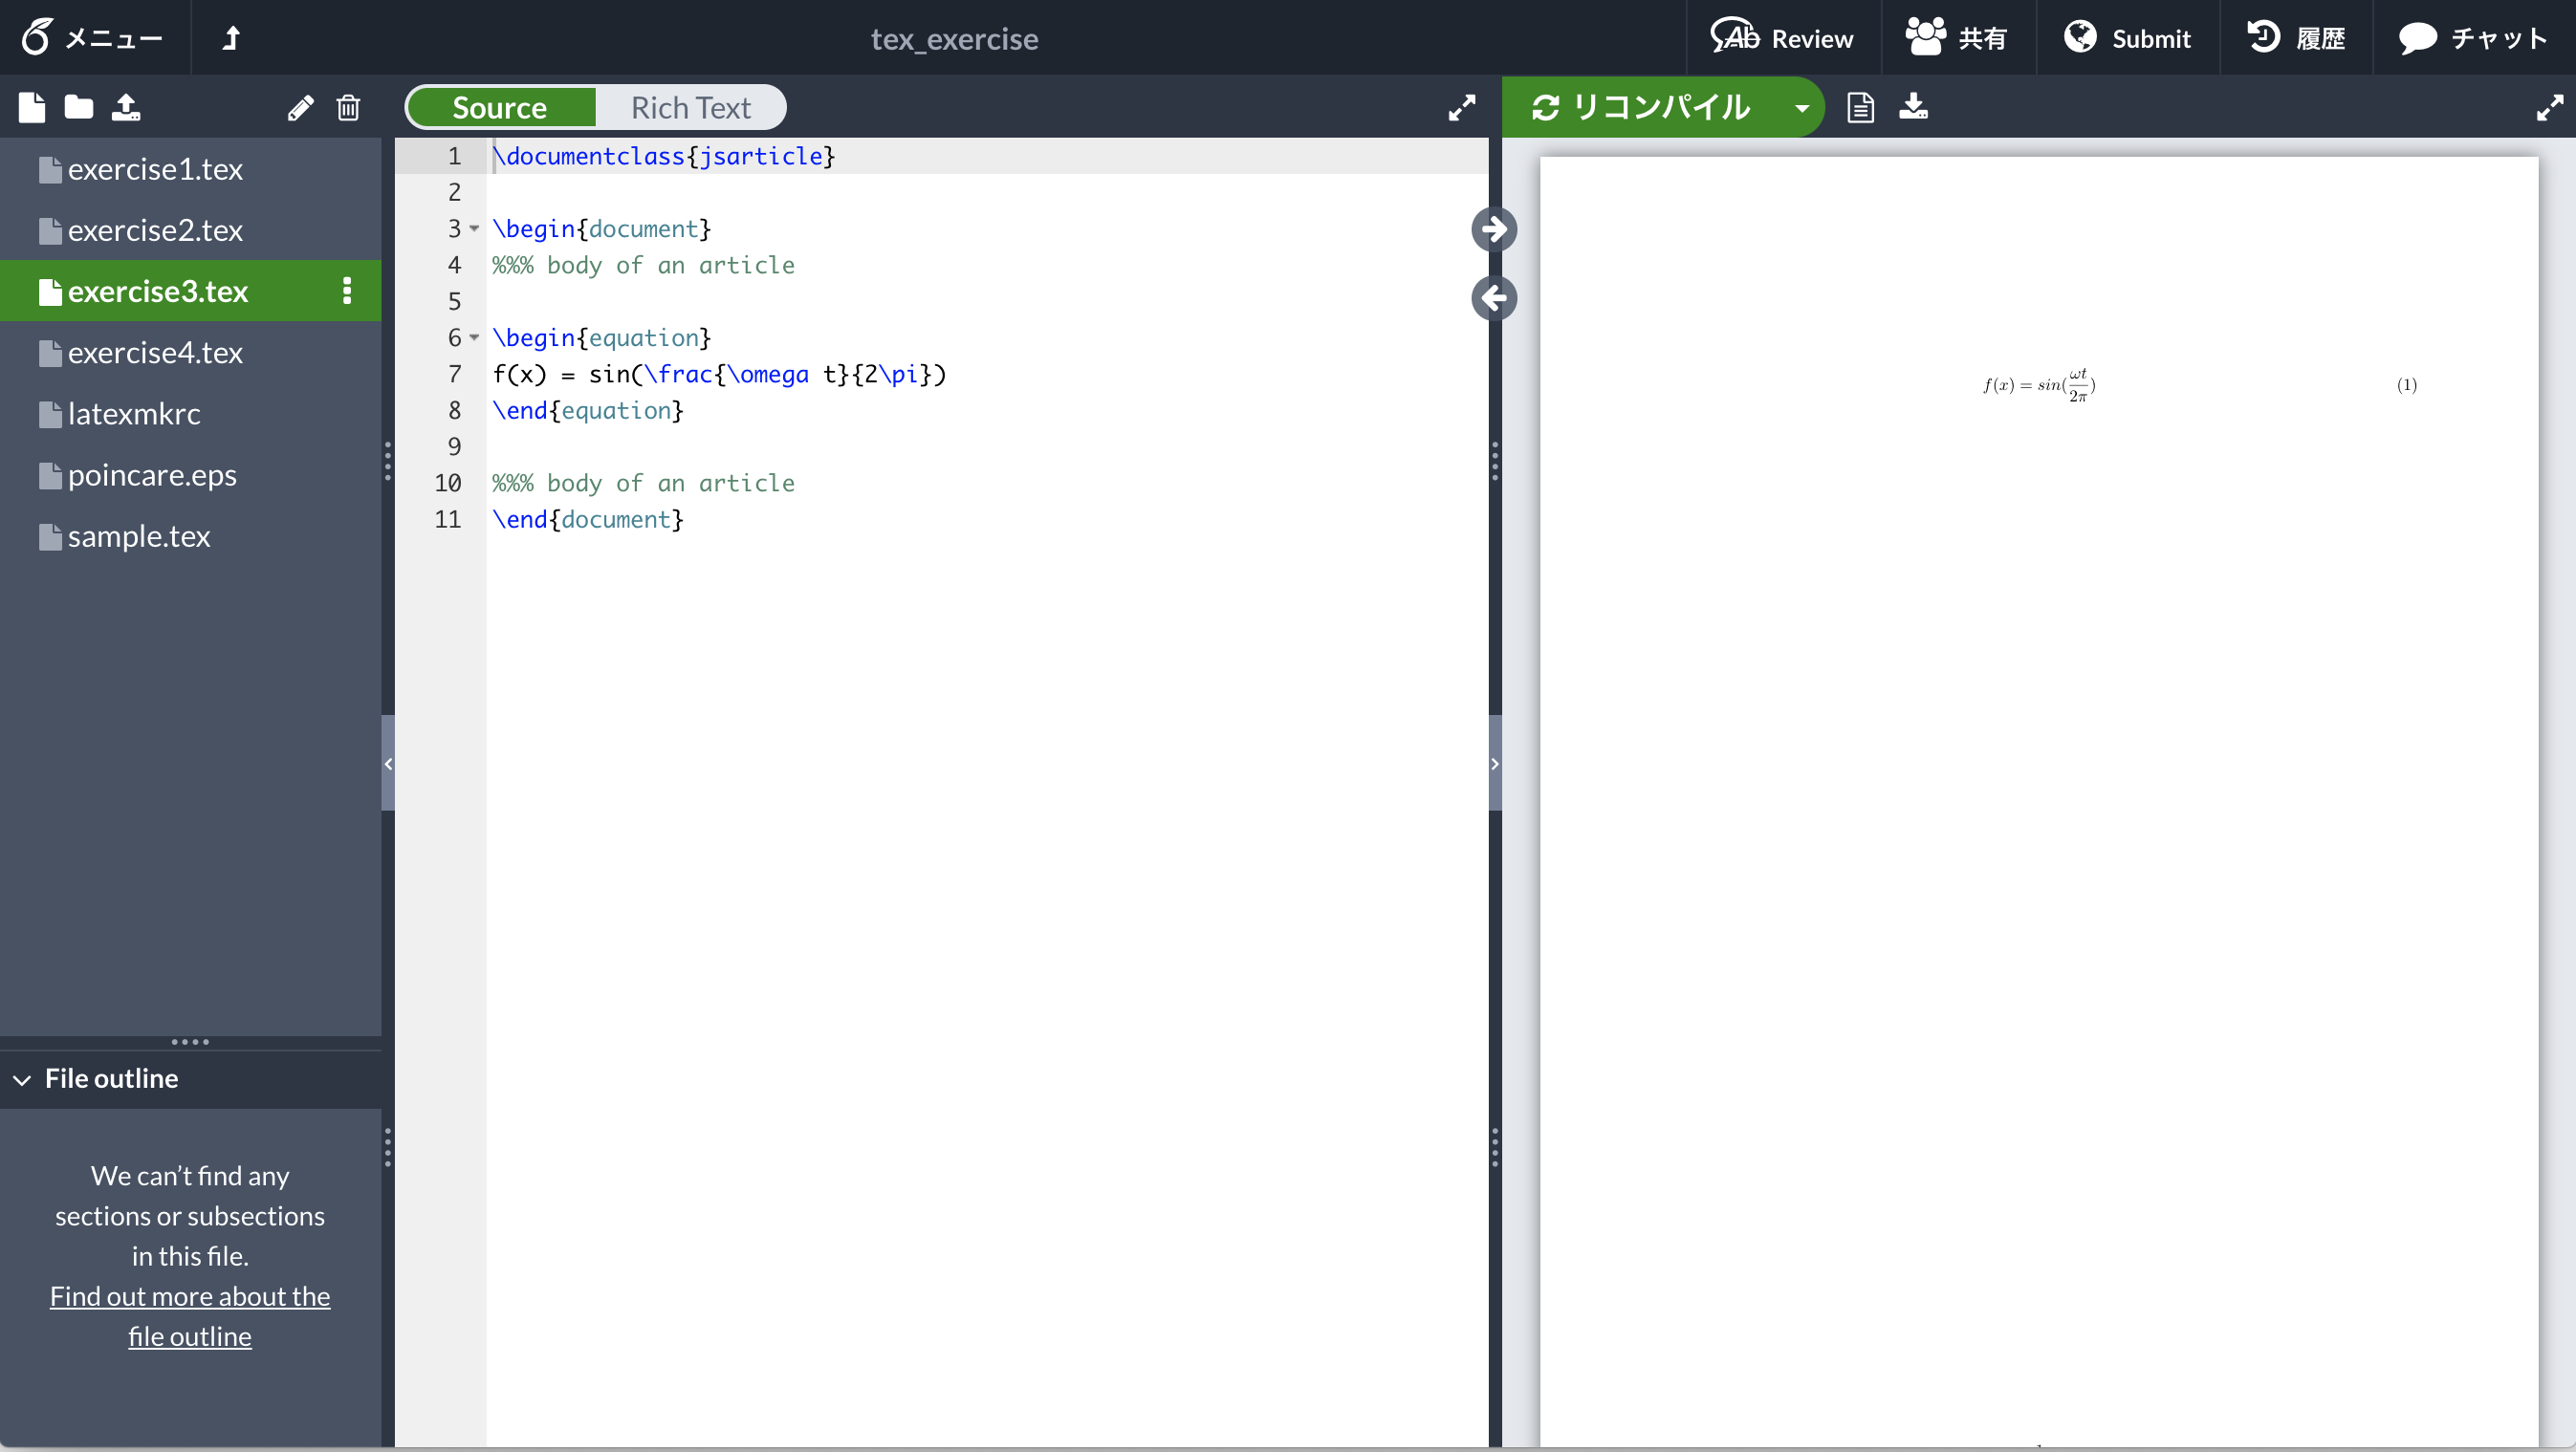
\includegraphics[width=100mm]{overleaf_start.png}
  \caption{\textbf{Overleaf}の作業画面}
  \label{overleaf}
\end{figure}
デフォルトでは日本語文章に対応していないため設定を変更しましょう。左上のメニューから\textbf{コンパイラ}で\textbf{LaTeX}を選択します。この設定と\underline{latexmkrc}という設定ファイルをプロジェクト内に置くことによって日本語文章を作成することができます。(今後別のプロジェクトで作業する際も同様の設定と、プロジェクト内にlatexmkrcを置いておくようにしましょう。)

\subsection{文章作成の流れ}
左上の\textbf{新規ファイル}からsample.texというファイルを作成し、左側のソースファイルの中身を次のようにします。
大文字・小文字も正確に入力してください。
\begin{screen}
\begin{verbatim}
\documentclass{jsarticle}
\begin{document}
こんにちは{\TeX}。はじめまして。
\end{document}
\end{verbatim}
\end{screen}

次に右枠上部の\textbf{リコンパイル}を押すことで、右側のプレビューに図\ref{hello}のように表示されます。これで文書の作成は完了です。

最後に右枠上部のダウンロードアイコンから作成したpdfファイルをダウンロードできます\footnote{メニューからソースファイルの一括ダウンロードもできます}。
このときファイル名はソースファイル名(sample)ではなくプロジェクト名(tex\_exercise)から取られます。
\begin{figure}
  \centering
  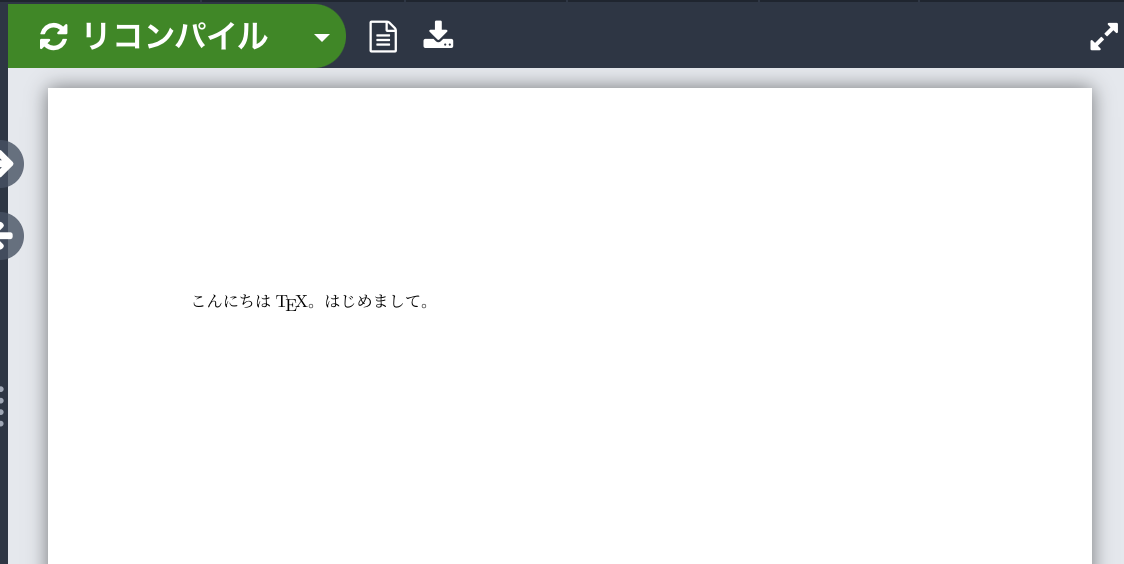
\includegraphics[width=100mm]{hellotex.png}
  \caption{pdfのプレビュー\label{hello}}
\end{figure}

\subsection{エラーに遭遇したら}
{\LaTeX}で文書を作成していると、しょっちゅうエラーに
遭遇します。このときの対処方法を覚えましょう。

先ほどのsample.texの2行目を少しだけ変えてみます。
\begin{screen}
\begin{verbatim}
\documentclass{jsarticle}
\began{document}
こんにちは{\TeX}。はじめまして。
\end{document}
\end{verbatim}
\end{screen}
これで\textbf{リコンパイル}を押すと図\ref{hello}とは異なる結果が表示されるでしょう。
このように思い通りに文章が作成されない時は再編集ボタンの右の\textbf{ログと出力ファイル}を見ます。
おそらく一つ目にこんなふうに言われていることでしょう。
\begin{screen}
\begin{verbatim}
Undefined control sequence. sample.tex, line 2

<recently read> \began

l.2 \began
          {document}
The control sequence at the end of the top line
of your error message was never \def'ed. If you have
misspelled it (e.g., `\hobx'), type `I' and the correct
spelling (e.g., `I\hbox'). Otherwise just continue,
and I'll forget about whatever was undefined.
\end{verbatim}
\end{screen}
こんなときは、表示された説明をよく読みます。今の場合は
\verb+begin+という
ところを\verb+began+と書いたため、怒られているようです。\verb+l.2+(2行目)
というのもヒントになりますね。さらに二つ目のログで
\begin{screen}
  \begin{verbatim}
LaTeX Error: Missing \begin{document}.
\end{verbatim}
\end{screen}
と言われているところからも原因を突き止めることができます。
こんな時はソースファイルに戻り、間違いを直してからもう一度\textbf{リコンパイル}を押します。
\pagebreak
